\section{手順}
\subsection{課題1}
\subsubsection{計測対象}
\begin{itemize}
  \item 計測対象である画像処理は、画像のノイズを除去することができる「
  3×3メディアンフィルタを使った平滑化」である。
  この実験では、図\ref{graph:1}のようなプログラムを使う。
  \item 画像処理に用いる画像は、「幅512ピクセル × 高さ479ピクセル」の図\ref{graph:2}のような
  画像である。
  \begin{figure}[hbtp]
    \begin{minipage}[t]{\hsize}   
      \centering
      \caption{メディアンフィルタを使った平滑化のプログラム}
      \label{graph:1}
      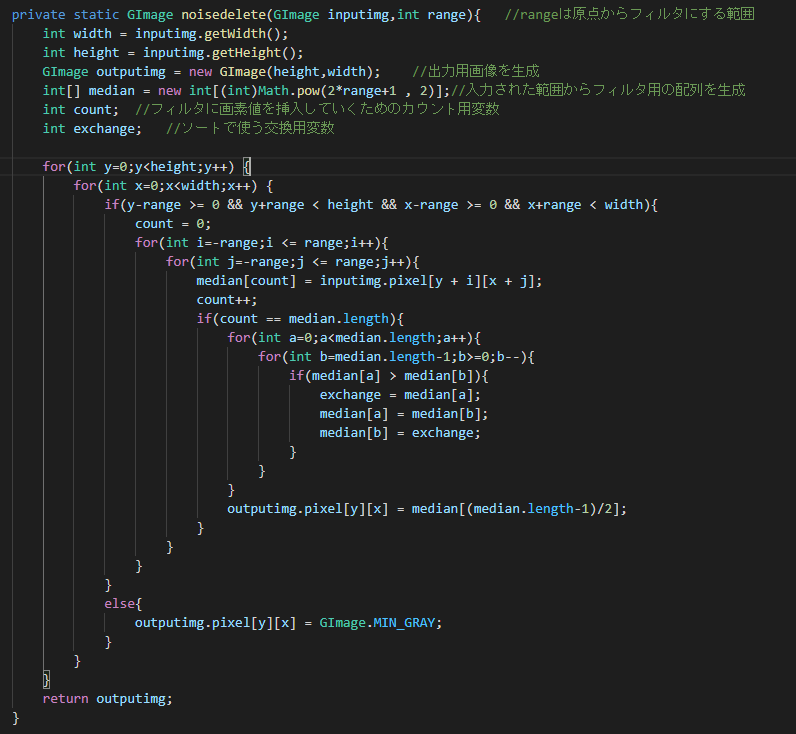
\includegraphics[scale = 0.75]{noisedeleteの中身1.PNG}
    \end{minipage}
    \begin{minipage}[t]{\hsize}
      \centering
      \caption{計測対象の画像処理に使う画像}
      \label{graph:2}
      \includegraphics[scale = 0.2]{d850429avhrr4.bmp}
    \end{minipage}
  \end{figure}
\end{itemize} 
\clearpage

\subsubsection{計測方法}
\begin{itemize}
  \item javaでは、「System.currentTimeMillis()」というメソッドを使うことで、long型で
  エポック秒から経過した時間をミリ秒単位で知ることができる。この実験では、
  このメソッドを用いて画像処理の処理時間を計測していく。
  \item 具体的な計測方法は「計測したい処理」を
  「System.currentTimeMillis()」で囲いこみ、処理後の時間から処理前の時間を引くことで
  、処理時間を計算する。
  \item 本題に入る前に、この計測方法が正確であるかどうかを
  確認する。javaの「Thread.sleep();」メソッドでは、引数に入れた数字×ミリ秒だけ、プログラムを
  一時停止することができる。これを利用して「Thread.sleep();」を処理とみなして、処理時間を
  計測し、「Thread.sleep();」の引数との比較を行うことで、計測方法が正確かどうかを判断する。
  \item この実験では、「Thread.sleep();」の引数を「1000」として、また、
  信頼性のあるデータをとるために、計測処理をfor文で20回繰り返えす図\ref{graph:5}のような
  プログラムを作成して計測した。その結果は、図\ref{graph:6}のようになり、結果をまとめると
  「1001ms」が9回、他は全て「1000ms」となった。1msの誤差が約1/2の確率で発生したが
  、この程度の誤差はマシンの性能などによる誤差の範疇だと考察できるため、
  この実験では、この計測方法は正確であると判断した。
  \item この実験では、画像処理の処理時間のみを正確に計測したいため、
  「System.currentTimeMillis()」を使って画像処理の処理時間を計測する前に、
  そもそもこの「System.currentTimeMillis()」という処理自体が時間を使っていないかを確認する。
  \item 計測方法は、図\ref{graph:3}のように、「System.currentTimeMillis()」を
  「System.currentTimeMillis()」で囲いこみ、処理後の時間から処理前の時間を引くことで
  、処理時間を計算する。また、信頼性のあるデータをとるために、これらの処理をfor文で
  20回繰り返している。
  \item 「System.currentTimeMillis()」の処理時間の計測結果は、図\ref{graph:4}の
  ように、試行回数20回の全てで「0ms」となった。これらの結果より、
  「System.currentTimeMillis()」の処理時間はこの実験では考慮しない。
  
  \begin{figure}[htbp]
    \begin{minipage}[t]{0.5\hsize}
      \centering
      \caption{「Thread.sleep();」を用いた計測方法の正確さ確認のプログラム}
      \label{graph:5}
      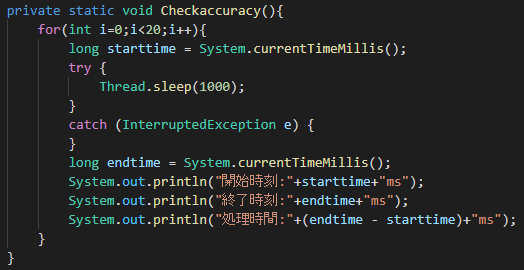
\includegraphics[scale=0.75]{計測方法の正確さを確認.PNG}
    \end{minipage}
    \begin{minipage}[t]{0.45\hsize}
      \centering
      \caption{「Thread.sleep();」を用いた計測方法の正確さ確認の出力結果}
      \label{graph:6}
      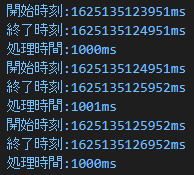
\includegraphics[scale=0.9]{計測方法の正確さを確認の出力.PNG}
    \end{minipage}
  \end{figure}
  \begin{figure}[htbp]
    \begin{minipage}[t]{0.5\hsize}
      \centering
      \caption{「System.currentTimeMillis()」の処理時間を計測するプログラム}
      \label{graph:3}
      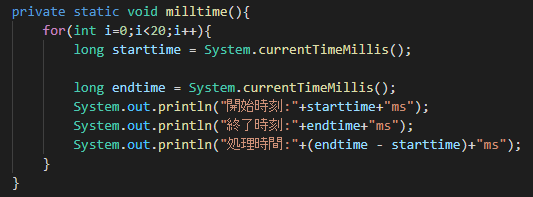
\includegraphics[scale=0.75]{milltimeのプログラム.PNG}
    \end{minipage}
    \begin{minipage}[t]{0.45\hsize}
      \centering
      \caption{「System.currentTimeMillis()」の処理時間の計測結果}
      \label{graph:4}
      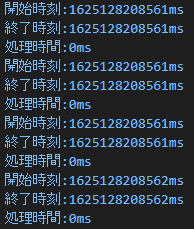
\includegraphics[scale=0.9]{milltimeの結果.PNG}
    \end{minipage}
  \end{figure}

\end{itemize}


\subsection{課題2}
\subsubsection{計測対象}
\subsubsection{計測方法}